\documentclass[12pt]{article}

\usepackage{hyperref}
\usepackage{natbib}
\bibpunct[: ]{(}{)}{;}{a}{}{,}
\usepackage[margin=1in]{geometry}
\usepackage{setspace} 
\usepackage{graphicx}
\usepackage{lscape}
\usepackage{subfigure}
\usepackage{authblk}
\renewcommand\Authfont{\normalsize}
\renewcommand\Affilfont{\footnotesize}

\hypersetup {
pdfauthor={Omar Lizardo},
pdfpagemode = UseNone,
pdfstartview=FitH,
citebordercolor = 0 1 0,
}

\begin{document}

\title{Variety in cultural choice and the instrumental use of social ties\thanks{A previous version of this paper was presented at the 2008 International Network for Social Network Analysis (INSNA) Sunbelt Conference in St. Pete's Beach, Florida and at colloquia at the University of Notre Dame and the University of Toronto. }}
\author[1]{Omar Lizardo}

\affil[1]{Deparment of Sociology, University of Notre Dame, 810 Flanner Hall, Notre Dame, IN, 46556.  \\ \url{olizardo@nd.edu}}

\date{\normalsize \today}

\maketitle


\newpage
\begin{abstract}
Building on the general connection between culture consumption and sociability which has been the focus of recent research in the sociology of culture, I propose that persons who have a propensity to consume a wide variety of cultural goods should also be observed to have successfully mobilized network ties for instrumental purposes, especially ``weak ties'' in contrast to ``strong ties.'' The results show that net of other individual predictors, as the cultural variety of the person's repertoire of tastes increases, there is 1) a higher likelihood of having activated a social tie to obtain information about jobs, and 2) a higher likelihood that the tie activation is through a weak, rather than strong ties or non-relational mechanisms.
\end{abstract}


\begin{center}
Word Count: 4,092
\end{center}

\doublespacing
\newpage 
\section{Introduction}
Recent research in the sociology of culture has argued and provided empirical evidence for the general proposition that culture consumption should be connected to networks of larger size, and that cultural variety, especially of cultural goods and experiences that are widely accessible and are spread fairly evenly across the social structure, is associated with the individual possession of social ties that span relatively larger distances in social space. Following this line of reasoning \citet[247]{erickson96} notes that ``[t]he more diverse the set of{\ldots}contacts one has, the more variety of culture one will encounter and hence maintain or learn{\ldots}Thus network variety is one important source of cultural variety.'' DiMaggio proposes that ``[t]he reason for this finding, so at odds with conventional notions about the isomorphism of taste and class{\ldots}, is that wide-ranging networks require broad repertoires of taste'' \citeyearpar[444]{dimaggio87}. \citet{lizardo06a} highlights the additional process of how tastes are \emph{converted} into a wider range of network ties. Thus, in the same way that network variety leads to cultural variety, having a wide-ranging repertoire of tastes is necessary to \emph{sustain} large networks over time, especially in the face of the large-scale volatility of personal relationships in contemporary social settings.  These are characterized by increasing pressures related to geographical mobility and other lifestyle choices that serve to recurrently disrupt network relations \citep{dimaggio96, dimaggio_mohr85, griswold_wright04, wellman_wortley90}.

This strand of research however, has so far ignored the fact that network theory focuses not only on relative differences in the size and density of individual networks---indexed by positional measures such as the various centrality indices \citep{freeman77, borgatti05}---but also on the relative \emph{resources} that are made available to individuals by virtue of having those ties \citep{bourdieu86, coleman88, portes98, lin01b}, and thus the differential opportunities to access those resources in times of need. In other words, networks are transformed from a potential store of benefits to actual\emph{ social capital} only in the process of agentic \emph{activation} of social ties \citep{lin99, lin00, lin01a, lin01b,mouw03, yakubovich05, lin_etal81a, lin_etal81b, lin_dumin86}.This activation can occur for the purposes of dealing with practical problems and issues like finding a job \citep{granovetter73} or obtaining  instrumental benefits in the form of material and emotional support from trusted contacts \citep{wellman_wortley90}. 

In this paper, I bring cultural capital theory and social capital theory into dialogue with another.  I do this by empirically examining the connection between \emph{culture consumption variety} \citep{dimaggio87, erickson96, peterson_rossman08} and network \emph{activation}.  I build on the general link between culture consumption and sociability which has been the focus of recent research in the sociology of culture \citep{bennett_etal99, witte_ryan04, cardon_granjon05, lizardo06a, jeannotte03} to propose some intuition of how the possession of cultural resources may lead to a higher likelihood of \emph{successful} activation of networks ties for instrumental purposes.

This paper is organized as follows: in the next section, I briefly review the literature on the sources and consequences of network activation. I then follow with a discussion of how we can use the general association between culture consumption and sociability in order to develop some theoretical intuition connecting culture consumption variety and the likelihood of using social networks to obtain valuable information. In the next section, I analyze data on the predictors of the prototypical form of network activation that has dominated the literature on social capital: using social networks to learn about job opportunities.  The results provide empirical evidence showing that culture consumption variety is positively tied to network activation:  net of other individual predictors, as the cultural variety of the individuals' repertoire of tastes increases, there is 1) a higher likelihood of activating social ties to obtain information about jobs, and 2) a higher likelihood that the tie activation is through a weak, rather than a strong tie. 

\section{Network ties as ``social capital''}
\subsection{Social capital as network diversity}
There are at least two primary ways in which social ties have been conceived as valuable in contemporary network theory and thus as a source of social capital.  The first has to do with the benefits that can be accrued from having a wide \emph{range} and \emph{diversity} of contacts \citep{burt82, burt83, burt92, lin_dumin86}. The conception of contact diversity as ``social capital'' relies on the well-established observation, first formulated in Granovetter's \citeyearpar{granovetter73} classic paper, that contact homogeneity in sociodemographic traits is associated with information \emph{redundancy}, while contact heterogeneity is associated with access to \emph{novel} sources of information. Whenever instrumental pursuits require access to novel sources of information---as when individuals use social contacts to learn about employment opportunities \citep{granovetter95}---those who are connected to diverse information sources will be more likely to learn about opportunities not otherwise accessible through the local network. Because extra-local information is more likely to be accessed through weak ties rather than strong ties, weak ties should provide the individual with an informational advantage not available to those embedded in local cliques. This is the ``strength of weak ties'' argument.

Studies of the association between social position and local network topology support the strength of weak ties argument. For instance, a well-established theme in network theory and research concern the long-standing association between socioeconomic status and the social diversity of contacts to whom the individual is connected. It is a well-established fact that higher status individuals are more likely to have social connections that span a wider distance in social space than low status individuals \citep{lin01a, lin01b}. 

An extensive variety of empirical evidence (mostly obtained through empirical examination of the ``core discussion network'') supports this contention. We know that the higher educated tend to have larger and less tightly knit (more likely to consist of persons not very well-acquainted with one-another) personal networks than the less educated \citep[129]{marsden87}.  Persons of higher education also tend to enjoy more diverse networks along such dimensions as gender and age \citep{fischer82}. Diversity in the local networks of high-status persons even extend to the \emph{kin network},with high status individuals displaying more heterogeneous kin networks (as measured by the standard deviation of educational attainment and occupational standing) than low status individuals \citep{goldstein_warren00}. In addition, a persons' occupational status (measured by scalar prestige indices) is positively associated both with the \emph{number} of social positions (defined as a detailed occupational classification) that the person is connected to (by having a friend in that job) as well as the \emph{range} of positions (as defined by the standard deviation of occupational prestige across the statuses) contained in their personal network (\citealp[90]{lin01b}; \citealp{lin_dumin86}). That is those of higher status are not only more likely to be connected to other persons of higher status, but are more likely to have social ties with persons of dissimilar status than are low status individuals.

\subsection{Social capital as access to resources}
The second way in which social connections have been conceived as ``social capital'' in network theory has to do with a factor that should be correlated with network diversity: the probability of having access to contacts that control or have access to desirable resources, such as influence, or who occupy high status positions.Thus, a big part of a person's status attainment process occurs through a relational pathway which partly mediated the resources obtained from the class of origins (father's or mother's education) and the individual's own attained status in determining current social position \citep{lin01a}.

A lack of local clustering (e.g. personal contacts being closely tied to one another) in the immediate social network is correlated with the \emph{resources}---as measured by the socio-demographic characteristics of alters---embedded in that network \citep{lin01a}. This explains why individual current achieved status is correlated with a lack of clustering, as measured by the range of positions accessible through the network.Thus, the individual's ascribed characteristics (resources from the family of origin) are associated with the pattern of network relations that he or she currently occupies. The volume of resources that corresponds to the individual's status or origin are positively associated with her current network structure and in part accounts for the association of current achieved status and local network structure \citep{lin90, lin01b}. 

In terms of Bourdieu's \citeyearpar{bourdieu86} theory of social capital, this is the process of ``conversion'' of educational and economic capital in the family of origin into current social capital.Social capital is converted into desirable resources by way of the agentic \emph{activation} of existing social ties. Thus, individuals derive advantage from relatively temporally stable qualities of their social network (size, diversity, rage, etc.) when they are able to call upon the resources embedded in that network as a result of situational contingencies (i.e. needing help finding a job). Thus, before being activated social capital remains in ``stasis'' as it where, and it is only by specific instance of network usage that we can get an empirical handle on the concept of social capital.

\section{Cultural capital and social networks}
A key analytical limitation of network theories of social capital is that they take the observed pattern of network connections as largely \emph{exogenous} to the analysis. That is, the fail to ask the question: where do social ties come from? Recent research at the intersection of the sociology of culture and network theory has begun to address this issue. In particular this research argues that insofar as social relationships are mediated through focused episodes of social interaction, and given that interaction rituals in modern societies tend to revolve primarily around the discussion of symbolic and cultural goods \citep{dimaggio87, dimaggio00} then individuals \emph{cultural tastes, competences and life-style practices,} should be a key predictor of both the size and range of personal networks.

The mobilization of cultural aptitudes and knowledge in conversation is clearly implicated in the \emph{capacity }of individual actors to constantly generate new social ties (and thus sustain a large and diverse social network over time). This insight acquires more salience when considered in the context of recent empirical confirmation of the short lived and ephemeral nature of most network connections \citep{bidart_degenne05, bidart_lavenu05, burt00, burt02, suitor_etal97, suitor_keeton97, feld_etal07}. This new strand of research therefore attempts to argue for the origins of the advantages produced by social network from the \emph{conversion} of cultural capital into social capital \citep{bourdieu86}. 

One of the primary ways in which tastes are used to sustain social networks, is by allowing the individual to connect to alters that are both relationally close---when specialist or (narrow) ``niche'' cultural tastes are concerned---and relationally distant---when talking about aptitude for broad-niche, or ``popular'' cultural forms \citep{lizardo06a}. Culture consumption and the ability to decode and appropriate symbolic goods produced are important resources that individuals mobilize in the \emph{construction} and \emph{maintenance} of active social relationships \citep{cardon_granjon05, dimaggio87, fine77}.  For the most part conversational interaction is devoted to discussion and commentary on symbolic goods \citep{fine77, dimaggio87}.This means that ``[m]any social relations are constructed, in different ways, around cultural and recreational activities'' \citep{cardon_granjon05}.This is an insight that harks back to classical process models of friendship formation, in with similarity based on cultural taste and practices \citep{mark98b}playing the role that ``value-homophily'' played in the original formulation \citep{lazarsfeld_merton54}. 

We should therefore expect that individuals who command a wide variety of tastes which cut across these well defined boundaries (i.e. those who have been referred to as ``omnivores'' in recent research \citep{peterson92, peterson05, peterson_rossman08}) and who will also be able to keep that high-variety taste pattern active over time---will also be more effective in sustaining high rates of social interaction in their---constantly shifting, sparse and loosely bounded---personal communities.  Lizardo \citeyearpar{lizardo06a} using data from the 2002 General Social Survey, finds empirical evidence consistent with this view. He finds that there is a monotonic relationship between the average size of the personal network (as measured by a one-shot item which asked the respondent the number of persons that the he or she comes into contact with at least once a year) and the number of cultural activities---associated with both the fine and the popular arts---that the respondent reports having engaged in at least once in the past year. In addition, the results of the analysis show that the number of as the number of cultural activities that the respondent engages in increases so does the expected size of their personal network, even after accounting for simultaneity bias. Thus it is clear that as culture consumption variety increases, access to larger (and by implication) more diverse social networks also increases \citep{dimaggio87, erickson96, lizardo06a}. 

\section{Empirical implications}
If the consumption of a variety of cultural goods is connected to the size and density of an individual's personal network \citep{dimaggio87, lizardo06a}, and if networks are a resource that is accessed when the individual requires either support, information or the projection of influence, we should expect those individual endowed with a more varied repertoire of tastes, to be able to sustain not only larger personal networks, but also to be relatively more likely to \emph{successfully access} those networks in a time of need. Thus, one empirical implication of the model proposed so far is that culture consumption variety should be connected with access of personal networks when individuals require information in comparison to non-relational forms of information search.

We should not only expect cultural taste variety to be connected to the use of relational pathways to information and influence.  More specifically, we should expect cultural variety to be connected to information access pathways that are \emph{more likely to be realized by the presence of a weak tie rather than a strong tie}. In the literature weak ties have been conceptualized in two different ways: 1) using a \emph{direct} measure of tie strength by counting weak ties as those named as ``acquaintances'' rather than close friends or relatives \citep{granovetter95, mouw03} and 2) using an \emph{indirect} measurement strategy, in which a persons is counted as having used a weak tie if they obtained their job by being contacted by the employer directly (without using an employment service or having answered and ad in the paper) \citep{yakubovich05}.  The rationale for the latter  (indirect measurement) strategy is that weak ties have been shown to serves as conduits of \emph{both} ``information and direct influence'' \citep[415]{yakubovich05}.The most frequent example of direct influence is of course a direct connection between the potential employer and the individual. It follows therefore that any factor that increases the probability of having a network richer in weak ties will increase the chances of any one individual already having a potential employer as an acquaintance \citep{yakubovich05}.  In either case, I hypothesize that if cultural variety and network variety are positively associated \citep{lizardo06a, erickson96}, and if network variety is defined as having a network rich in contacts who are different from ego, and who are therefore more likely to be weak ties, we should expect that cultural variety will increase the chances of individuals having potential employers as acquaintances, and of thus mobilizing those weak ties when necessary. 

\section{Data and Variables}
I use data from the culture and network modules of the 2002 General Social Survey (Davis, Smith and Marsden, 2002). The GSS is administered biannually by the National Opinion Research Center (NORC) to a nationally representative sample of non-institutionalized, English-Speaking American adults. The 2002 wave of the GSS contained a recurring module on participation in the arts (similar to ones fielded in 1993 and 1998), along with a new module related to social networks and social support. The network module contained a question asking the respondent to report the \emph{method} that they used to obtain their last job, which, in conjunction with the self-report measures of cultural participation, makes these data suitable for testing the hypotheses outlined above.

\subsubsection{Cultural variety scale}
Respondents were asked to report whether they had engaged in the following activities during the past year: 1) gone to see a movie in a theater 2) gone to a live performance of popular music like rock, country, or rap 3) gone to a live performance of a non-musical stage play 4) attended a live ballet or dance performance 5) gone to a classical music or opera performance and 6) visited an art museum or gallery and 7) read a novel, poem or play. The variables are coded one if the respondent engaged in that activity in the past year and zero otherwise. As a measure of cultural variety, I create a linear index (Cronbach's $\alpha=0.93$) that equals the total number of cultural activities (ranging from zero to seven) that the respondent reported engaging in the last year.  This is what \citep{warde_etal08} have referred to as ``omnivorousness by volume.'' Previous research validates the criterion validity of this type of measure as an indicator of consumption patterns characteristic of young, upwardly mobile elites \citep[e.g.][]{bryson96, sullivan_katzgerro07, warde_etal08}.

\subsubsection{Network activation indicator}
This is measured through an item that asked the respondents to ``\emph{indicate how you first [from whom] found out about work at your present employer}'' respondents who were not currently working were asked to answer this question for their last job.  In what follows I limit the analysis to currently employed respondents.\footnote{A separate category was reserved for people who had never participated in the labor force.} I recode the original variable into a polytomous item containing seven categories.  These are shown in Table~\ref{tab1a}.\footnote{Respondents coded as having answered ``Don't Know'' are not considered in the analysis.} About 44\% of respondents found out about their job from a social contact (either through relatives, close friends or acquaintances). However, and consistent with previous research and theory, among respondents who did use a social contact, respondents were more than twice as likely to rely on a strong tie (relatives or close friends) in comparison to using an acquaintance.  Although if we count both acquaintances and direct contact as weak ties and relatives and close friends as strong ties, then respondents are only one and a half time more likely to rely on the latter relational mechanism in comparison to the former.

\section{Results}
\subsection{Means-difference tests}
Are there differences in the extent to which persons engage in more extensive patterns of culture consumption for different respondent categories (divided according to the method through which they found out about their jobs)?  To answer this question, I regress the cultural variety scale against dummy-variable indicators of whether the respondent found out about their current job using the seven job-search methods shown in the first column of Table~\ref{tab1} (in addition to the ``don't know'' category).  The \emph{t}-test corresponding to whether the coefficient in this bivariate regression is significantly different from zero, is equivalent to a test of whether average number of cultural activities engaged in differ for a given group of respondents in comparison to the rest of the sample.  The results are shown in the last four columns of Table~\ref{tab1}.

What I find is broadly consistent with expectations.  Respondents who found out about their job through a strong tie (close friends) display narrower taste profiles than the average respondent ($t=-2.46, p<0.05$).  Respondents who learned about their current job through kin ties are no different from the rest in terms of their culture consumption behavior ($t=-0.48$).   Consistent with expectations,  respondents who relied on contact information from a weak tie (e.g. an acquaintance) have \emph{broader} than average cultural variety scores ($t=2.03, p<0.05$), as do respondents who were themselves contacted directly by the employer ($t=3.14 p<0.01$).   This reflects two different sources of network embeddedness, roughly consonant between the difference between ``outdegree'' (social capital as a result of knowing lots of others) and ``indegree'' (social capital as a result of being known by lots of others) in network analysis.  Both of these have been argued to be connected to the mobilization of weak ties over strong ties \citep{granovetter95, yakubovich05}.\footnote{Respondents who used the non-relational method of calling or asking themselves or simply answering a sign or and ad display more restricted taste patterns than average, but neither of these differences reach conventional levels of statistical significance.  None of the other contrasts are statistically significant. }   

\subsection{Multivariate analysis}
It is possible that the results shown in Table~\ref{tab1} are the spurious by-product of unobserved socio-demographic heterogeneity among persons with different cultural breadth profiles.  For instance, if the highly educated are more likely to use weak-ties to find a job (or to be directly contacted by the employer), and they are also more likely to consume culture then the difference in the cultural variety score between those who found out about their current job through and acquaintance and the rest of the sample might simply be due to differences in education and not the higher likelihood of those who consume a variety of culture to be better connected.  The same argument can be made via heterogeneity premised on age, gender or race.  

I use probit regression models for binary outcomes to account for these sources of possible spuriousness.  I specify a regression equation predicting the odds of having found out about the current job through one of the mechanisms listed in Table~\ref{tab1}.  In the probit model, the observed binary dependent variable ($y=0,1$) is considered to be the empirical realization of a continuous, unbounded, latent underlying variable ($-\infty \geq y^{*} \leq \infty$).  We observe distinct categorical realizations of this underlying variable only if $y^{*}$ falls below or above a certain threshold.  The relationship between the latent normal variates ($y^{*}$) and the observed binary variables ($y$) is as follows:

\begin{equation}
y=g(y^{*})=\left\{
        \begin{array}{rl}
                0 &\mbox{if $y^{*} \leq 0$} \\
                1 &\mbox{if $y^{*} > 0$}
        \end{array}\right.		
        \label{eq1}
\end{equation}


\begin{equation}
	y^{*}_{i}=\alpha+\sum{\beta_{k} x_{ik}}+u_{i}
\end{equation}

Where $\beta_{k}$ is a vector of unknown regression coefficients, and $u_{i}$ is a classical (identically and normally distributed) disturbance with expected value zero and standard deviation of one.  Table~\ref{tab2} shows the results of a series of binary probit models in which the dependent variable equals one if the respondent used one of the search methods considered above, and zero otherwise.  I use the cultural variety scale as a predictor, but estimate the effect while adjusting for the respondent's education, age, gender, status as a racial or ethnic minority (classification as either African-American or Hispanic).  I also control for the occupational prestige of the current occupation (relevant if members of high and low status occupations are disproportionately more likely to rely on certain job-search methods\citep{mouw03}).

The results show that after adjusting for the most plausible socio-demographic confounders the differential likelihood of those respondents who consume a wide variety of cultural goods to have obtained a job by reliance through particular \emph{socially embedded} mechanisms remains.  Respondents who have high scores in the cultural variety scale are more likely to have used a information from an acquaintance to learn about their current job ($t=2.19$) or to have been contacted by their current employer directly ($t=2.61$) suggesting that these persons are ``better connected'' than respondents who do not consume a wide variety of culture.  

In fact, the cultural variety scale is the \emph{best} individual predictor of the likelihood of having learned about the current job through an acquaintance; none of the other individual-level covariates reaches conventional levels of statistical significance ($t<|1.96|$).\footnote{This means that the bivariate model (the one including only cultural variety as a predictor) does a good of a job of statistical prediction as the model including the vector of controls ($p<0.05$).}  When it comes to predicting who learns about their job by being contacted by the employer, only age is a better predictor than the cultural variety score.   

The only result shown in Table~\ref{tab1} that appears to be due to socio-demographic heterogeneity separating ``omnivore'' culture consumers from their ``univore'' counterparts is that corresponding to using a strong tie to find a job.  After controlling for the relevant socio-demographic characteristics, I find that high cultural variety respondents are no more or less likely to have found out about their job through a close friend than persons with more restricted tastes ($t=-0.82$). More specifically, racial and ethnic minorities ($t=2.13$) and married respondents ($t=3.03$) are more likely to have learned about their job from a close friend.  These two respondent categories are also less likely to be cultural omnivores ($p<0.05$; results not shown).\footnote{In addition, I find that adjusting for variation in socio-demographic characteristics brings to light a result that was {\em suppressed} in Table~\ref{tab1} due to unspecified heterogeneity:  high cultural variety individuals are much less likely than chance to have found their job through the (non-relational) means of having called themselves ($t=-1.98$).}

We have found that persons who consume a wide variety of culture are more likely to have found their current job through two distinct mechanisms associated with the use of weak ties:  information from an acquaintance or direct contact from their current employer.  While both of these types of respondents can be said to consume on average a wider variety of cultural goods than respondents who used other relational and non-relational mechanisms to learn about their current job, it is possible that their patterns of cultural choice differ systematically.  To explore this issue, I estimated separate probit regression models predicting the odds of having used these two job search methods but using the binary indicator for each type of culture consumption as a predictor (not the overall cultural variety scale).  This means that I estimated fourteen regression models (seven binary components of the cultural variety scale for each of the two job search outcomes).

The results of this analysis are summarized in Figure~\ref{fig1}.  In the figure, I plot the marginal effect \citep[126]{long_freese06} corresponding to the binary culture consumption indicator on a given job-search method outcome.  The marginal effect gives the average shift in the probability of observing a respondent fall into a given job search class, given that we ``turn-on'' that binary indicator of culture consumption from its null value of zero to one. 

The figure shows that respondents who found their job using the two ``weak tie'' mechanisms have distinct culture consumption profiles.  In particular, genres that are better classified as ``popular culture''---they have less socio-demographically restricted audiences as given by the expected educational attainment of consumers---help us predict whether a person used an acquaintance to learn about their job, but do not help us in predicting whether they were contacted directly by their current employer.  More elite cultural genres on the other hand, do a good job in predicting who  obtained their current employment by being contacted directly but do not help us in identifying respondents who used acquaintances to learn about their current job.\footnote{The only exception is reading, which is not an elite genre, but which also does not have much of an impact in predicting who used an acquaintance to learn about their job.}  

This suggests that popular culture consumption is associated with the mobilization of existing weak ties \citep{lizardo06a}, while being contacted directly by the employer is closer to a signal of being embedded in favorable position in more elite social circles \citep{kadushin66}.

\section{Discussion and Conclusion}
The above results provide support for the proposition that at least some of the value of cultural variety in contemporary American society is \emph{social}: the ability to appropriate a wide variety of symbolic goods allows the individual to maintain---and diachronically replenish \citep{cardon_granjon05, lazarsfeld_merton54}---\emph{a larger} and \emph{a more varied} personal network.   Persons who engage in a variety of cultural activities are more likely to have successfully mobilized a socially embedded strategy when looking for a job, in particular those involving the activation of \emph{weak ties} but not those involving the activation of strong or embedded ties.  Most importantly this tie mobilization appears to reflect precisely the type of network advantages that are associated with cultural variety: the activation of weaker arms-length relationships. These are precisely those relationships which in certain contexts---such as the loosely-knit networks of constantly shifting relationships associated typical of high-status Euro-American Westerners---that are most likely to produce advantages in the labor market (by for instance providing information about high-paying jobs or jobs that provide more of a fit between personal competences and qualifications and actual task activities). 

In addition, I find that while engaging in a wide variety of activities increases the chances of engaging not all cultural activities have the same functional linkage to network activation. Activities closer to the category of ``popular culture'' (e.g. mass disseminated via ``culture-industry systems'') appears to increase the chances of having successfully learned about the current job via an acquaintance; this is consistent with ``culture conversion'' arguments that point to the elective affinity between popular culture and weak-tie formation and maintenance processes \citep{lizardo06a}.  Activities associated with the higher prestige fine and performance arts, on the other hand, appear to be associated with having been contacted directly by the employer. While both of these can be considered prototypical ``weak-tie'' activation episodes, they differ in the underlying phenomenology and mechanism:  the first is to be expected of individuals who have networks rich in fleeting acquaintances directed by themselves towards others (outdegree) while the latter is characteristic of individuals who are likely to be known or sought out by a large number of potential contacts (indegree). Omnivores---who consume both popular and high status culture---may thus be able to enjoy \emph{both} of these network advantages when exploiting social resources for instrumental purposes. In this manner cultural variety affords the person with resource complementarity as manifested in both lots of outgoing ties directed to the person \emph{toward} diverse others and in lots of connections coming to the individual \emph{from} others, most importantly those located in positions of influence or authority \citep{yakubovich05, bian97, podolny_baron97}.

This analysis contributes to our understanding of the role of culture in processes of stratification by connecting culture consumption variety not only to the static \emph{possession} of virtual resources in the form of larger and more varied networks of social relations, but by providing empirical evidence of a link between culture consumption variety and the likelihood of attaining desirable outcomes through the \emph{activation} of personal relationships.  This is important because it is through the activation of resources embedded in social relations that social capital is theorized as going from a potential to a real resource \citep{lin99, lin01a}. These results are consistent with the general proposition that cultural taste variety ``counts'' as cultural capital in contemporary social settings precisely due to the intimate association of culture consumption and sociability.  Heterogeneity in the opportunities and likelihood to engage in this type of sociable interaction, can then be traced differences in rates of engagement in culture consumption \citep{witte_ryan04}.  This points to the building of social relationships through face-to-interaction as mediated by cultural content as one of the key mechanisms linking cultural stratification and status attainment outcomes.



\singlespacing
\newpage
\bibliographystyle{asr}
\bibliography{N:/Private/zotero-library}
\end{document}

%Figures
\newpage
\begin{figure}[htb!]
	\centering
		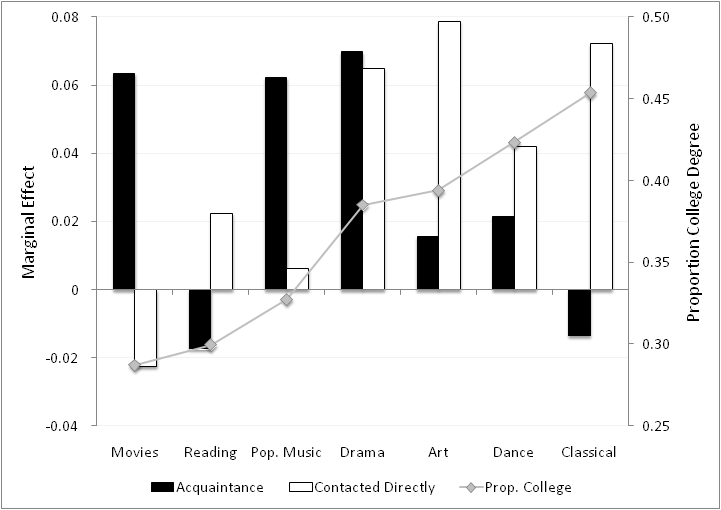
\includegraphics[height=4.2in]{line-bar.png}
		\caption{Marginal effects of genre-specific cultural consumption on the likelihood of having used two different job search methods with horizontal sorted by the average education of consumers of those genres, 2002 GSS.}
	\label{fig1}
\end{figure}


%Tables
\newpage
\begin{table}[ht!]
\caption{Proportion of respondents in each job search category, 2002 General Social Survey, analysis restricted to currently employed respondents (full-time or part-time), $N=720)$}
\begin{tabular*}{\hsize}{@{\extracolsep{\fill}} r l c} 
\hline
\hline
& Job Search Method & Sample Prop.\\
\hline
	1& From a relative &10.8\%\\
	2& From a close friend &20.0\%\\
	3& From an acquaintance &14.3\%\\
	4& From a placement service (school, public or private)&11.2\%\\ 
	5& From an advertisement or a sign &17.5\%\\ 
	6& Directly contacted by employer &11.0\%\\ 
	7& Called the employer or asked myself in person&15.0\%\\
\hline
\end{tabular*}
\label{tab1a}
\end{table}


\newpage
\begin{table}[ht!]
\caption{Mean cultural variety scale differences by job search method category, 2002 General Social Survey, analysis restricted to currently employed respondents (full-time or part-time), $N=720)$}
\begin{tabular*}{\hsize}{@{\extracolsep{\fill}} l*{7}{c}} 
\hline
\hline
&\multicolumn{2}{c}{Mean N. Cultural Activities}&&\\
&$\beta=0$&$\beta=1$&\emph{t}-statistic&\emph{p}-value\\
\hline
Relatives&2.49&2.40&-0.48&0.629\\
Close Friend&2.55&2.19&-2.46&0.014\\
Acquaintance&2.43&2.78&2.03&0.043\\
Emp. Service&2.46&2.67&1.14&0.255\\
Advertisement/Sign&2.51&2.33&-1.19&0.233\\
Directly From Employer&2.41&3.01&3.14&0.002\\
Called/Asked Myself&2.51&2.30&-1.29&0.196\\
\hline
\end{tabular*}
\label{tab1}
\end{table}

\newpage
\begin{landscape}
\begin{table}[htb!]
\caption{\footnotesize Binary probit models predicting job search method, 2002 General Social Survey.  (1) Relatives , (2) Close Firend, (3) Acquaintance, (4) Emp. Service/School , (5) Advertisement/Sign , (6) Direct Contact with Employer, (7) Called/Asked Myself; , analysis restricted to currently employed respondents (full-time or part-time).}
\begin{tabular*}{\hsize}{@{\extracolsep{\fill}} l*{7}{c}} 
\hline
\hline 
&(1)&(2)&(3)&(4)&(5)&(6)&(7)\\
\hline
Cultural Variety Scale   &     0.03&    -0.03&     0.09&    -0.02&    -0.07&     0.11&    -0.08\\
                         &   (0.62)&  (-0.82)&   (2.19)&  (-0.56)&  (-1.63)&   (2.61)&  (-1.98)\\
N. of Years of Education &    -0.02&    -0.02&    -0.02&     0.02&    -0.01&     0.03&     0.04\\
                         &  (-0.53)&  (-0.89)&  (-0.79)&   (0.73)&  (-0.55)&   (0.96)&   (1.43)\\
Occ. Prestige (Current Job)&    -0.02&    -0.01&    -0.00&     0.02&     0.01&    -0.00&     0.00\\
                         &  (-3.11)&  (-1.73)&  (-0.38)&   (3.23)&   (1.90)&  (-0.70)&   (0.27)\\
Respondent's Age         &    -0.02&     0.00&    -0.00&    -0.01&    -0.00&     0.02&     0.01\\
                         &  (-3.70)&   (0.01)&  (-0.40)&  (-0.91)&  (-0.94)&   (4.13)&   (1.60)\\
Gender (Women=1)         &    -0.15&    -0.12&     0.06&    -0.02&     0.06&     0.11&     0.05\\
                         &  (-1.09)&  (-1.05)&   (0.50)&  (-0.12)&   (0.56)&   (0.81)&   (0.43)\\
Race/Eth. (Black or Hispanic=1)&    -0.57&     0.33&    -0.05&     0.12&    -0.17&     0.24&    -0.02\\
                         &  (-2.58)&   (2.13)&  (-0.30)&   (0.64)&  (-1.02)&   (1.30)&  (-0.13)\\
Mar. Status (Married=1)  &     0.02&     0.36&     0.10&    -0.13&    -0.20&     0.22&    -0.34\\
                         &   (0.12)&   (3.03)&   (0.77)&  (-0.90)&  (-1.69)&   (1.60)&  (-2.68)\\
N. of Children           &     0.02&    -0.08&     0.01&    -0.03&     0.10&    -0.05&     0.03\\
                         &   (0.31)&  (-1.79)&   (0.12)&  (-0.59)&   (2.25)&  (-0.99)&   (0.76)\\
City Size in 1000s (logged)&     0.01&    -0.01&     0.04&    -0.01&     0.03&     0.00&    -0.06\\
                         &   (0.39)&  (-0.39)&   (1.16)&  (-0.42)&   (1.13)&   (0.04)&  (-1.93)\\ \\
Model $\chi^{2}$                     &    39.75&    27.27&     7.53&    22.24&    13.76&    32.08&    18.77\\ \\
N                        &   \multicolumn{7}{c}{717}\\
\hline
\end{tabular*}
\label{tab2}
\end{table}


\end{landscape}

\end{document}

















